%%%%%%%%%%%%%%%%%%%%%%%%%%%%% Define Article %%%%%%%%%%%%%%%%%%%%%%%%%%%%%%%%%%
\documentclass[addpoints]{exam}
%%%%%%%%%%%%%%%%%%%%%%%%%%%%%%%%%%%%%%%%%%%%%%%%%%%%%%%%%%%%%%%%%%%%%%%%%%%%%%%

%%%%%%%%%%%%%%%%%%%%%%%%%%%%% Using Packages %%%%%%%%%%%%%%%%%%%%%%%%%%%%%%%%%%
\usepackage{amsmath}
\usepackage{amssymb}
\usepackage{geometry}
\usepackage{venndiagram}
\usepackage{graphicx}
\usepackage{float}
\usepackage[breaklinks]{hyperref}
\usepackage{listings}
\usepackage{pdfpages}
\usepackage{comment}
\usepackage{empheq}
\usepackage{mdframed}
\usepackage{booktabs}
\usepackage{lipsum}
\usepackage{color}
\usepackage{wrapfig}
\usepackage{bookmark}
\usepackage{titlesec}
\usepackage{hyperref}
\usepackage{parskip}
\usepackage{empheq}
\usepackage{verbatim}
\usepackage{subfig}
%%%%%%%%%%%%%%%%%%%%%%%%%%%%%%%%%%%%%%%%%%%%%%%%%%%%%%%%%%%%%%%%%%%%%%%%%%%%%%%

% Other Settings

%%%%%%%%%%%%%%%%%%%%%%%%%% Page Setting %%%%%%%%%%%%%%%%%%%%%%%%%%%%%%%%%%%%%%%
\geometry{a4paper}
\printanswers
\qformat{}

%%%%%%%%%%%%%%%%%%%%%%%%%% Define some useful colors %%%%%%%%%%%%%%%%%%%%%%%%%%
\definecolor{ocre}{RGB}{243,102,25}
\definecolor{mygray}{RGB}{243,243,244}
\definecolor{deepGreen}{RGB}{26,111,0}
\definecolor{shallowGreen}{RGB}{235,255,255}
\definecolor{deepBlue}{RGB}{61,124,222}
\definecolor{shallowBlue}{RGB}{235,249,255}
%%%%%%%%%%%%%%%%%%%%%%%%%%%%%%%%%%%%%%%%%%%%%%%%%%%%%%%%%%%%%%%%%%%%%%%%%%%%%%%

%%%%%%%%%%%%%%%%%%%%%%%%%% Define an orangebox command %%%%%%%%%%%%%%%%%%%%%%%%
\newcommand\orangebox[1]{\fcolorbox{ocre}{mygray}{\hspace{1em}#1\hspace{1em}}}
%%%%%%%%%%%%%%%%%%%%%%%%%%%%%%%%%%%%%%%%%%%%%%%%%%%%%%%%%%%%%%%%%%%%%%%%%%%%%%%

%%%%%%%%%%%%%%%%%%%%%%%%%%%%%%% Title & Author %%%%%%%%%%%%%%%%%%%%%%%%%%%%%%%%
\title{Operating Systems - CS/CE 232L/324L\\ Lab 13: Using Signls to Communicate Between Processes}
\author{Ali Muhammad Asad - aa07190}
\date{} %Leave uncommented if u want automatic date which is done through maketitle, else u can uncomment this and type anything else u want over here - not necessary to enter a date over here
%%%%%%%%%%%%%%%%%%%%%%%%%%%%%%%%%%%%%%%%%%%%%%%%%%%%%%%%%%%%%%%%%%%%%%%%%%%%%%%

\begin{document}
\maketitle

\begin{center}
    \gradetable[h]
\end{center}

\vspace*{5mm}
\begin{questions}
    \question
    \textbf{Question 1:} How did you stop the code in section 3?
    \begin{solution}
        Since the process was going on forever, and \texttt{Ctrl+C} wasn't working, I opened a new terminal, and ran the \texttt{``top''} command. This effectively showed me a list of the processes running at that time. I then found the process ID of the process I wanted to terminate, and then ran the command \texttt{``kill -9 <PID>''} to kill the process. The command \texttt{``kill -SIGTERM <PID>''} could also be used.
        \begin{figure}[H]
            \centering
            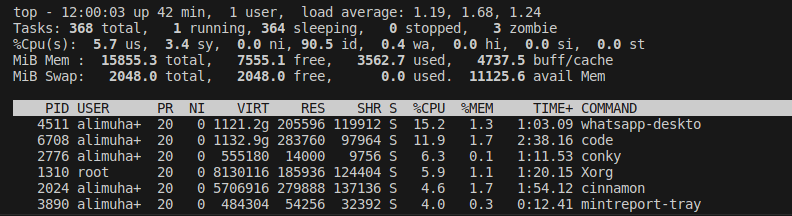
\includegraphics[width=1.0\textwidth]{top.png}
        \end{figure}
        The image depicts a list of processes when \texttt{``top''} was run [the process in question vanished by the time since sleep had been called, but it was noted]. The command was then run; command in question \texttt{``kill -9 16503''}. When the command was run, the process was terminated as shown below: 
        \begin{figure}[H]
            \centering
            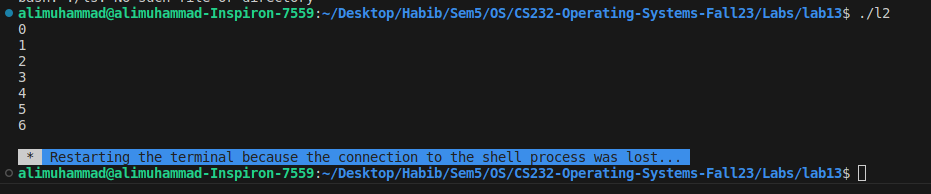
\includegraphics[width=1.0\textwidth]{end.png}
        \end{figure}
    \end{solution}

    \question
    \textbf{Question 2:} How do we use signal function in section 3?
    \begin{solution}
        The \texttt{signal(arg1, arg2)} function in section 3 is used to define how a program handles different signals, essentially interrupts or notifications sent to a process by the OS. The first argument is of type \texttt{int}: the signal that we want to handle. For eg, \texttt{SIGINT} is the signal number for the interrupt signal generated when we press \texttt{Ctrl+C}. The second argument is of type \texttt{void (*func)(int)}: the function that we want to run when the signal is received. In our section, \texttt{SIG\_IGN} is used to ignore the signal. The return type is of type \texttt{void (*func)(int)}: a pointer to the previous signal handler for the specified signal. 
    \end{solution}

    \question
    \textbf{Question 3:} Try converting void signal\_handler function in section 4 to a return function. What happened if you do that. Explain why did that happen.
    \begin{solution}
        I changed the function to a static int to return an integer, a character type to return a char, and a double to return a double.
        My compiler did issue some warnings when I compiled the program, however, the behavious did not change when I ran the program. This could be since the expected signature for a signal handler function is void. So by changing the return type, it no longer matches the expected signature as per convention. Signal handling is meant to be a quick response, so signal handlers are designed to return `void'. The fact that the behaviour didn't change is an example of how undefined behaviour can manifest in C. The return type is not used by the system. Since the operating system's signal dispatching mechanism doesn't do anything with a return value from a signal handler, returning an int instead of void has no practical effect. 
    \end{solution}

    \question
    \textbf{Question 4:} In lab exercise, try interrupting the terminal before the quit/exit is called in the code.
    \begin{solution}
        This keeps on running since the child process keeps on ignoring the interrupt signal, much as it was happening in section 4 (same reasoning). 
    \end{solution}

    % \textbf{Question 5:} For Exercise, in Child process, print your first name and in parent process print your second name and student ID. Delay the parent process from execution till the time reaches is the same number of seconds as the sum of first 2 digits of your student ID.
    % \begin{solution}
        
    % \end{solution}
    
\end{questions}
\end{document}